
\documentclass[11pt]{article}

% ------------------------------------------------------------
% Packages
% ------------------------------------------------------------
\usepackage[margin=1in]{geometry}
\usepackage[T1]{fontenc}
\usepackage{lmodern}
\usepackage{pdflscape}
\usepackage{longtable}
\usepackage{microtype}
\usepackage{amsmath,amssymb,mathtools}
\usepackage{booktabs}
\usepackage{array}
\usepackage{graphicx}
\usepackage{caption}
\usepackage{subcaption}
\usepackage{enumitem}
\usepackage{xcolor}
\usepackage{hyperref}
\usepackage{setspace}
\usepackage{natbib}
\usepackage{threeparttable}

\hypersetup{
    colorlinks=true,
    linkcolor=blue,
    citecolor=blue,
    urlcolor=blue
}

\setlength{\parindent}{0pt}
\setlength{\parskip}{0.72em}
\onehalfspacing

% ------------------------------------------------------------
% Title information
% ------------------------------------------------------------
\title{\textbf{Insulin Resistance and Systemic Inflammation Below the HbA1c Prediabetes Threshold:}\\
\textbf{Age-Dependent Associations in U.S. Adults, NHANES 2015--March 2020}}


% ------------------------------------------------------------
% Document
% ------------------------------------------------------------
\begin{document}

\author{
Scott Moerschbacher$^{1}$,
Janice Baker$^{1,2}$
}

\date{}
\maketitle

\begin{center}
$^{1}$Open Inquiry Research Group, USA\\
$^{2}$Department of Sociology, University of Nevada, Reno,
Reno, Nevada, USA
\end{center}

\vspace{1em}

% ============================================================
\begin{abstract}

\textbf{Background:}
Insulin resistance may be present despite glycemic measures remaining below
conventional thresholds for prediabetes, but whether its relationship with
systemic inflammation varies across adulthood is unclear. We examined the
association between the Homeostatic Model Assessment of Insulin Resistance
(HOMA-IR) and high-sensitivity C-reactive protein (hs-CRP) among adults with
HbA1c $<5.7\%$ and tested whether this association was modified by age.

\textbf{Methods:}
We conducted a cross-sectional analysis of 3,079 adults aged $\geq20$ years
without diagnosed diabetes and with HbA1c $<5.7\%$ using harmonized
pre-pandemic NHANES 2015--March 2020 data. Survey-weighted regression models
estimated associations between HOMA-IR and log-transformed hs-CRP while
adjusting for HbA1c, waist circumference, continuous age, sex, and non-HDL
cholesterol. Effect modification was evaluated using a formal
HOMA-IR-by-age-group interaction for ages 20--39, 40--54, and $\geq55$
years. Independent-cycle analyses, continuous-age modeling, and multiple
sensitivity analyses evaluated reproducibility and robustness.

\textbf{Results:}
The HOMA-IR--hs-CRP association differed across age groups
($F(2,40)=5.69$, $p=0.00671$). A one-unit higher HOMA-IR was associated
with approximately 2.7\% higher hs-CRP among adults aged 20--39 years
($\beta=0.0266$; 95\% CI, 0.0038--0.0495) and 5.2\% higher hs-CRP among
those aged 40--54 years ($\beta=0.0511$; 95\% CI, 0.0132--0.0890).
Among adults aged $\geq55$ years, the association was attenuated and not
statistically distinguishable from zero ($\beta=-0.0189$; 95\% CI,
$-0.0513$--0.0135). Survey-weighted median HOMA-IR was similar across age
groups, indicating that the interaction was not simply attributable to
higher average HOMA-IR in midlife. The age-dependent pattern was broadly
supported by independent-cycle analyses, continuous-age modeling, and
sensitivity analyses, although the strength of formal interaction evidence
varied across model specifications.

\textbf{Conclusions:}
Among U.S. adults without diagnosed diabetes and with HbA1c below the
conventional prediabetes threshold, the adjusted association between
HOMA-IR and systemic inflammation varied across age. These findings suggest
that adults with HbA1c $<5.7\%$ remain metabolically heterogeneous and that
variation in insulin resistance may provide information about inflammatory
physiology not captured by glycemic classification alone. Prospective
studies are needed to determine whether measuring insulin resistance adds
clinically useful information to conventional glycemic assessment and
whether such utility varies with age.

\end{abstract}

\section{Introduction}

Glycohemoglobin (HbA1c) plays a central role in the identification of
dysglycemia and diabetes risk. Because it reflects cumulative glycemic
exposure over preceding weeks to months \citep{Nathan2007}, HbA1c provides clinically useful
information about glucose regulation and is incorporated into widely used
diagnostic thresholds for prediabetes and diabetes \citep{ADA2026Diagnosis}. Glycemic status,
however, is not synonymous with insulin sensitivity. During the development
of insulin resistance, compensatory increases in insulin secretion may
preserve circulating glucose concentrations despite diminished tissue
responsiveness to insulin \citep{Rodzen2026}. Individuals who remain below conventional HbA1c
thresholds may therefore occupy different metabolic states despite sharing
the same glycemic classification.

The homeostatic model assessment of insulin resistance (HOMA-IR), derived
from fasting glucose and fasting insulin concentrations, provides a
surrogate estimate of insulin resistance and captures information not
contained in HbA1c alone \citep{Matthews1985,Wallace2004}. Although HOMA-IR is not a direct physiological
measurement of insulin sensitivity, it is well suited to large population
studies in which more intensive methods such as the
hyperinsulinemic-euglycemic clamp are not feasible \citep{DeFronzo1979,Wallace2004}. The coexistence of
relatively normal glycemia with higher fasting insulin and HOMA-IR therefore
provides one plausible form of metabolic heterogeneity beneath conventional
glycemic thresholds.

Insulin resistance is also embedded within a broader network of metabolic
and inflammatory processes. Adipose tissue dysfunction, altered lipid
handling, hepatic metabolism, and immune signaling are closely interconnected
with insulin action, while inflammatory pathways can themselves influence
insulin signaling \citep{Park2014AgingIR,Chen2004,Park2009,Yan2019}.
High-sensitivity C-reactive protein (hs-CRP), an acute-phase protein
produced primarily by the liver in response to inflammatory signaling,
provides a nonspecific marker of systemic inflammatory activity
\citep{Pepys2003}. An association between HOMA-IR and hs-CRP would not
establish a causal relationship between insulin resistance and inflammation,
but could indicate that variation in insulin resistance is associated with
physiologically relevant inflammatory heterogeneity.

Previous population-based studies have established associations between
insulin resistance and systemic inflammatory markers in adults without
diabetes. Analyses of U.S. NHANES data and other population cohorts have
reported positive associations between HOMA-IR or fasting insulin and
C-reactive protein after adjustment for demographic, anthropometric, and
metabolic covariates
\citep{Chen2004,Meng2007,Park2009,Missel2021}.
Related work has demonstrated metabolic and inflammatory heterogeneity even
within populations without overt diabetes or conventional hyperglycemia
\citep{Caporaso2020}.

More recently, \citet{Shahid2023} examined HOMA-IR and C-reactive protein
in a nationally representative Canadian population without diabetes and
considered potential heterogeneity by sex and age. However, that study
included participants with HbA1c values extending through the conventional
prediabetes range ($<6.5\%$), whereas the present study restricts the
primary population to HbA1c $<5.7\%$. Its principal findings also centered
on sex rather than the age-dependent association examined here. Similarly,
\citet{Caporaso2020} examined HOMA-IR across demographic and metabolic
strata in a broader NHANES population but did not focus on formal age
modification of the HOMA-IR--CRP relationship among adults restricted to
HbA1c below 5.7\%.

Collectively, these studies establish that the relationship between insulin
resistance and inflammation is not itself a new observation. However,
comparatively little population-based evidence has addressed whether age
modifies the HOMA-IR--hs-CRP association specifically among adults who
remain below the conventional HbA1c prediabetes threshold of 5.7\%.

This question is relevant to recent calls for improved recognition and
characterization of insulin resistance before the development of overt
metabolic disease. \citet{Rodzen2026}, in a recent narrative review,
highlighted the absence of standardized clinical criteria for insulin
resistance and called for improved diagnostic frameworks and further
research to support earlier identification. Importantly, they also
emphasized the heterogeneity of insulin resistance and the need to interpret
surrogate measures within appropriate clinical and physiological contexts.
Their framework raises an empirical question relevant to glycemic
classification: among individuals who remain below conventional glycemic thresholds, does a
measure of insulin resistance provide biologically relevant information not
captured by glycemic classification alone?

In this context, we use the term metabolic screening ``blind spot'' in a
limited sense. The term does not imply that HbA1c is an inadequate measure
of glycemia, that individuals with HbA1c below 5.7\% are necessarily
metabolically unhealthy, or that HOMA-IR should replace established
screening measures. Rather, it refers to the possibility that classification
based on glycemia alone may leave meaningful variation in insulin resistance
unresolved among individuals assigned to the same glycemic category. If
that variation is systematically associated with inflammatory status, then
glycemic classification and insulin-resistance measures may provide
complementary information about metabolic phenotype.

The National Health and Nutrition Examination Survey (NHANES) provides an
opportunity to examine this question in a nationally representative U.S.
population with simultaneous measurements of HbA1c, fasting glucose,
fasting insulin, anthropometry, lipids, and hs-CRP \citep{Akinbami2022NHANES}. In the present study,
we used harmonized pre-pandemic NHANES data from 2015 through March 2020 to
examine adults aged 20 years or older without diagnosed diabetes and with
HbA1c below 5.7\%. The original study hypothesis was that HOMA-IR would be
associated with systemic inflammatory status within this population,
consistent with metabolic heterogeneity not captured by glycemic
classification alone.

During methodological evaluation of the initially observed age-stratified
associations, age emerged as a potential effect modifier. The revised
analysis therefore formally evaluated the HOMA-IR-by-age interaction using
a pooled survey-weighted model rather than inferring effect modification
from differences in statistical significance across separately fitted age
strata. The age-dependent pattern was subsequently evaluated using
continuous nonlinear modeling of age, independent-cycle replication,
alternative outcome and exposure transformations, anthropometric
specifications, inflammatory restrictions, and additional sensitivity
analyses. Accordingly, the present study addresses both the original
question of whether HOMA-IR is associated with inflammatory heterogeneity
below the conventional HbA1c prediabetes threshold and the subsequently
identified question of whether that association varies across adulthood.

% ============================================================

\section{Methods}

\subsection{Study Design and Data Source}

We conducted a cross-sectional analysis of publicly available data from the
National Health and Nutrition Examination Survey (NHANES), using the
2015--2016 cycle and the 2017--March 2020 pre-pandemic data release.
NHANES is a nationally representative survey of the noninstitutionalized
U.S. population that combines interviews, physical examinations, and
laboratory measurements using a complex, multistage probability sampling
design \citep{NHANES2017_2020Guidelines}.

The 2015--2016 and 2017--March 2020 datasets were harmonized at the
participant level using the NHANES participant identifier (\texttt{SEQN}).
Variables required for the present analysis were obtained from the
demographic, examination, diabetes questionnaire, glycohemoglobin,
fasting glucose, fasting insulin, high-sensitivity C-reactive protein,
and lipid files. Because HOMA-IR requires both fasting glucose and fasting
insulin, analyses were conducted within the NHANES fasting laboratory
subsample and used the corresponding fasting-subsample survey weights.

The primary analysis combined the available pre-pandemic observations
from 2015 through March 2020. The two conventional 2015--2016 and
2017--2018 NHANES cycles were additionally analyzed separately as an
independent-cycle replication analysis \citep{NHANES2017_2020Guidelines}.


\subsection{Analytic Population}

The analytic population was restricted to adults aged 20 years or older
who had no self-reported diagnosis of diabetes and had HbA1c $<5.7\%$,
the lower boundary of the conventional HbA1c-defined prediabetes range
\citep{ADA2026Diagnosis}. Participants were additionally required to belong
to the qualifying NHANES fasting laboratory subsample, as indicated by a
nonzero fasting-subsample survey weight, and to have valid fasting glucose
and fasting insulin measurements, positive HOMA-IR and hs-CRP values, and
complete data for variables included in the primary harmonized model. No
imputation of missing data was performed.

Fasting-subsample eligibility was independently verified using
participant-reported fasting duration from the NHANES fasting
questionnaire, calculated as
\texttt{PHAFSTHR} + \texttt{PHAFSTMN}/60
\citep{NHANESFasting2015,NHANESFasting2017_2020}.
All participants with a qualifying fasting-subsample weight in the
final analytic population reported fasting durations within the
NHANES qualifying range of 8 to $<24$ hours, confirming concordance
between fasting-subsample eligibility and reported fasting duration.

Of 3,182 participants meeting the remaining eligibility and measurement
requirements, 103 (3.2\%) were excluded because of incomplete primary-model
covariate data, yielding a final primary analytic sample of 3,079
participants (Supplementary Figure~S1). The final sample represented
approximately 144.3 million U.S. adults after application of the combined
survey weights.

No a priori sample-size calculation was performed; the analytic sample
comprised all participants from the specified NHANES survey periods who
met the study eligibility criteria and had the data required for the
primary analysis.

The HbA1c restriction was used to examine metabolic heterogeneity
specifically among individuals remaining below the conventional laboratory
threshold for prediabetes. This restriction defines the population under
study and should not be interpreted as establishing that all included
participants were otherwise metabolically healthy.

\subsection{Exposure: HOMA-IR}

The primary exposure was the Homeostatic Model Assessment of Insulin
Resistance (HOMA-IR), a surrogate measure of insulin resistance derived
from fasting insulin and fasting glucose concentrations
\citep{Matthews1985,Wallace2004}. HOMA-IR was calculated as

\[
\mathrm{HOMA\!-\!IR}
=
\frac{
\mathrm{fasting\ insulin}\;(\mu\mathrm{U/mL})
\times
\mathrm{fasting\ glucose}\;(\mathrm{mg/dL})
}{405}.
\]

HOMA-IR was modeled continuously and retained on its original scale in the
primary analysis. Although HOMA-IR was right-skewed, log transformation of
the exposure did not materially improve residual behavior when hs-CRP was
modeled on the log scale. Retaining HOMA-IR on its original scale also
permits direct interpretation of model coefficients per one-unit difference
in HOMA-IR. Log-transformed HOMA-IR was evaluated in sensitivity analyses.


\subsection{Outcome: hs-CRP}

The primary outcome was high-sensitivity C-reactive protein (hs-CRP),
modeled as its natural logarithm,

\[
Y=\ln(\mathrm{hsCRP}).
\]

Raw hs-CRP exhibited substantial right skew and produced strongly skewed
and heavy-tailed regression residuals. Log transformation markedly improved
residual behavior and was therefore selected for the primary model on
statistical-distributional grounds rather than on the basis of statistical
significance.

For models using $\ln(\mathrm{hsCRP})$, coefficients were converted when
useful to proportional differences on the original hs-CRP scale according to

\[
100\left(e^\beta-1\right)\%.
\]

Models using untransformed hs-CRP were retained as sensitivity analyses.


\subsection{Age and Covariates}

Following the methodological evaluation of the initial age-stratified
findings, age was designated as the primary effect modifier in the revised
analysis. For the principal analysis and presentation, participants were
classified into three age groups:

\[
20\text{--}39,\qquad
40\text{--}54,\qquad
\geq55\text{ years}.
\]

Age was also retained as a continuous covariate within the adjusted model
to account for within-category age variation. The categorical age groups
were selected to provide interpretable estimates of effect modification;
sensitivity analyses treated age continuously and allowed the HOMA-IR
association to vary nonlinearly across adulthood.

The primary harmonized adjustment set consisted of HbA1c, waist
circumference, continuous age, sex, and non-HDL cholesterol. Non-HDL
cholesterol was calculated as

\[
\mathrm{non\!-\!HDL}
=
\mathrm{total\ cholesterol}
-
\mathrm{HDL\ cholesterol}.
\]

Waist circumference was selected as the primary anthropometric covariate
because it was consistently available across the survey periods included
in the combined analysis and provides a measure of central adiposity.
This choice was also consistent with NHLBI guidance identifying waist
circumference as a practical anthropometric measure of abdominal adiposity
and a better marker of abdominal fat content than waist-to-hip ratio
\citep{NHLBI1998Obesity}. Waist-to-hip ratio was not used in the primary
combined-period model because hip circumference was not available
consistently across all included survey periods.

\subsection{NHANES Survey Design and Weighting}

All population estimates and inferential analyses incorporated the NHANES
complex sampling design \citep{NHANES2017_2020Guidelines}. Because calculation of HOMA-IR required both
fasting glucose and fasting insulin, analyses were conducted within the
qualifying NHANES fasting laboratory subsample and used the corresponding
fasting-subsample survey weights rather than general examination weights.

Fasting-subsample eligibility was independently verified using
participant-reported fasting duration from the NHANES fasting questionnaire,
calculated as \texttt{PHAFSTHR} + \texttt{PHAFSTMN}/60. All participants
with a qualifying fasting-subsample weight in the final analytic population
reported fasting durations within the NHANES qualifying range of 8 to
$<24$ hours, confirming concordance between fasting-subsample eligibility
and reported fasting duration.

Survey variance estimation additionally incorporated the NHANES masked
variance stratum (\texttt{SDMVSTRA}) and masked variance unit
(\texttt{SDMVPSU}) variables \citep{NHANES2017_2020Guidelines}. These variables account for the stratified
and clustered public-use survey design and were used for variance estimation
rather than as biological covariates.

For the combined 2015--March 2020 analysis, fasting weights were adjusted
for the unequal durations represented by the component datasets according to the NHANES guidance \citep{NHANES2017_2020Guidelines}. The
2015--2016 fasting weight was rescaled as

\[
W_{15/16}^{*}
=
\mathrm{WTSAF2YR}
\left(\frac{2}{5.2}\right),
\]

and the 2017--March 2020 pre-pandemic fasting weight as

\[
W_{17/20}^{*}
=
\mathrm{WTSAFPRP}
\left(\frac{3.2}{5.2}\right).
\]

Masked variance strata and variance units were uniquely identified across
periods before the datasets were combined. The resulting combined design
provided 40 survey design degrees of freedom.

Survey-design-based variance estimates were used for standard errors,
confidence intervals, $t$-tests, and $F$-tests. Participants were therefore
not treated as independent simple-random-sample observations.


\subsection{Primary Statistical Analysis}

The primary analysis estimated the adjusted association between HOMA-IR
and log-transformed hs-CRP and formally tested whether that association
differed across age groups. The model can be represented as

\[
\begin{aligned}
\ln(\mathrm{hsCRP}_i)
={}&
\beta_0
+\beta_1 H_i
+\boldsymbol{\beta}_2 A_i
+\boldsymbol{\beta}_3(H_i\times A_i)
+\boldsymbol{\gamma}^{T}Z_i
+\epsilon_i,
\end{aligned}
\]

where $H_i$ denotes HOMA-IR, $A_i$ denotes age group, and $Z_i$ contains
HbA1c, waist circumference, continuous age, sex, and non-HDL cholesterol.

The primary inferential test was the joint survey-adjusted test of

\[
H_0:
\beta_{\mathrm{HOMA},20-39}
=
\beta_{\mathrm{HOMA},40-54}
=
\beta_{\mathrm{HOMA},55+}.
\]

Thus, evidence for effect modification was determined from the
HOMA-IR-by-age interaction itself rather than by comparing whether
independently estimated age-specific coefficients crossed a conventional
significance threshold.

Age-specific HOMA-IR slopes and their 95\% confidence intervals were
subsequently estimated from the fitted interaction model to characterize
the direction and magnitude of the association within each age group.

For comparison with the primary adjusted estimates, unadjusted
age-specific HOMA-IR associations were also estimated in the same
complete-case analytic population using the survey-weighted
HOMA-IR-by-age-group model without the primary adjustment covariates;
survey period was retained as a nuisance term in the combined-period
analysis.

For the combined-period analysis, a survey-period indicator was included,
and the adjustment covariates---HbA1c, waist circumference, continuous age,
sex, and non-HDL cholesterol---were permitted to have period-specific
coefficients through interactions with survey period. The
HOMA-IR-by-age-group association remained the common effect-modification
structure of primary interest. This specification avoided unnecessarily
assuming that nuisance covariate relationships were identical in the
2015--2016 and 2017--March 2020 components.

Several design and analytic features were used to reduce potential bias. NHANES fasting-subsample survey weights were applied to account for the complex sampling design and differential probability of selection into the fasting subsample. Eligibility and exposure definitions were applied consistently across survey periods, and the primary model used harmonized covariates available across the full study period. Sensitivity and replication analyses were used to evaluate the robustness of the observed age-dependent association to alternative model specifications, outcome and exposure scales, survey periods, and additional potential confounders. As an independent cross-software validation, the primary analysis and selected sensitivity analyses were reimplemented from the raw NHANES files in R using the survey package. Analytic sample construction, survey design degrees of freedom, model estimates, age-specific contrasts, and joint Wald statistics reproduced the primary Python implementation to numerical precision.

\subsection{Independent-Cycle Replication}

To assess reproducibility independently of the expanded combined analysis,
harmonized models were fitted separately to the conventional 2015--2016
and 2017--2018 NHANES cycles. Within each cycle, the HOMA-IR-by-age
interaction and corresponding age-specific slopes were estimated using the
appropriate fasting-subsample weights and survey-design variables.

Replication was evaluated from the consistency of estimated age-dependent
patterns and by a formal HOMA-IR-by-age-group-by-cycle interaction testing
whether age-specific HOMA-IR associations differed between cycles.
Statistical significance of an age-specific coefficient in one cycle and
nonsignificance in another was not, by itself, considered evidence of
between-cycle heterogeneity.


\subsection{Continuous-Age Analysis}

To evaluate whether the categorical age findings depended on the selected
age boundaries, age was additionally modeled continuously. We examined
linear and quadratic HOMA-IR-by-age interactions and a natural cubic spline
representation of age using four degrees of freedom.

The spline model estimated the adjusted HOMA-IR slope as a continuous
function of age,

\[
\beta_{\mathrm{HOMA}}(a)
=
\frac{
\partial E[\ln(\mathrm{hsCRP})\mid X]
}{
\partial\,\mathrm{HOMA\!-\!IR}
},
\]

where $a$ denotes age.

This analysis was used to assess the shape of age modification rather than
to identify a discrete biological age threshold. In particular, crossing of
the estimated slope or its confidence interval through zero was not
interpreted as defining a specific age at which the HOMA-IR--hs-CRP
association begins or ends.


\subsection{Sensitivity Analyses}

Sensitivity analyses were organized according to the potential source of
inferential vulnerability they were intended to address rather than treated
as additional primary analyses.

Because HbA1c was used both to define the analytic population
(HbA1c $<5.7\%$) and as a continuous adjustment covariate in the primary
model, we additionally repeated the primary analysis without continuous
HbA1c adjustment while retaining the HbA1c eligibility criterion. This
analysis assessed whether conditioning on residual within-range variation
in HbA1c materially influenced the estimated HOMA-IR--hs-CRP association
or its modification by age.

\paragraph{Outcome distribution and inflammatory extremes.}
We repeated analyses using untransformed hs-CRP and examined models
restricting hs-CRP to $\leq10$ mg/L to assess sensitivity to observations
potentially reflecting acute inflammatory states. The inflammatory-restriction
analysis was evaluated using both log-transformed and untransformed hs-CRP
outcomes.

\paragraph{Exposure scale.}
We evaluated log-transformed HOMA-IR in combination with both raw and
log-transformed hs-CRP. Together with the primary specification, these
analyses formed a four-model transformation grid evaluating raw and log
scales for both exposure and outcome.

\paragraph{Age specification.}
In addition to the primary categorical interaction, HOMA-IR effect
modification was evaluated using continuous linear age, quadratic age,
and a four-degree-of-freedom natural cubic spline representation.

\paragraph{Adiposity specification.}
Because adiposity is closely related to both insulin resistance and
systemic inflammation, the dependence of the primary findings on the
anthropometric specification was examined explicitly. Waist circumference
remained the harmonized primary adiposity measure. The primary model was
refitted using BMI and waist-to-height ratio in place of waist circumference.
These comparisons were additionally performed in a common analytic sample
with complete data for all three measures to distinguish differences due to
anthropometric specification from differences in sample composition.
Waist-to-hip ratio was evaluated separately during the survey period in
which hip circumference was available, with comparisons among waist
circumference, BMI, waist-to-height ratio, and waist-to-hip ratio restricted
to the same participants.

\paragraph{HbA1c eligibility.}
Additional sensitivity analyses progressively relaxed the HbA1c eligibility
criterion from $<5.7\%$ to $<6.0\%$, $<6.5\%$, and no HbA1c restriction
while continuing to exclude participants with diagnosed diabetes. These
analyses were used to assess whether the observed age-dependent pattern,
particularly attenuation among older adults, could be explained primarily
by the original HbA1c selection threshold.

\paragraph{Survey-cluster and influence analyses.}
Survey-cluster influence was evaluated using a leave-one-cluster-out
procedure in which each unique masked stratum--PSU combination was removed
in turn and the primary model refitted. Additional influence analyses
examined the sensitivity of results to influential HOMA-IR and hs-CRP
observations and to restrictions on extreme values.

\paragraph{Additional supportive analyses.}
Where the required variables were available and scientifically appropriate,
additional analyses evaluated smoking, medication burden, statin use,
renal and liver/metabolic biochemical variables, expanded covariate sets,
and sex heterogeneity. These analyses were considered supportive or
exploratory rather than additional primary hypothesis tests and were not
uniformly available across the full harmonized study period.


\subsection{Descriptive Statistics and Statistical Inference}

Characteristics of the primary analytic population were summarized overall
and by age group. Approximately symmetric continuous variables were
reported as survey-weighted means with standard errors. Because fasting
insulin, HOMA-IR, and hs-CRP were strongly right-skewed, these variables
were summarized using survey-weighted medians and interquartile ranges.

Regression coefficients are reported with survey-adjusted standard errors,
95\% confidence intervals, and two-sided $p$-values where appropriate.
Joint interaction hypotheses were evaluated using survey-adjusted $F$-tests.
A conventional two-sided $\alpha=0.05$ threshold was used as a reference
for statistical inference; however, interpretation considered effect
magnitude, confidence intervals, consistency across analyses, and the
distinction between primary and sensitivity analyses rather than treating
$p=.05$ as a strict boundary between the presence and absence of an
association.


\subsection{Statistical Software and Computational Implementation}

Data management and statistical analyses were performed in Python
(version 3.13.5). Data manipulation was conducted using pandas
(version 2.2.3), numerical matrix operations using NumPy
(version 2.3.5), regression design matrices using patsy
(version 1.0.2), and statistical distribution functions using SciPy
(version 1.17.0).

Survey-weighted regression coefficients were estimated directly using
weighted least squares. For a design matrix $\mathbf{X}$, outcome vector
$\mathbf{y}$, and diagonal matrix of survey weights $\mathbf{W}$, the
coefficient estimator was

\[
\widehat{\boldsymbol{\beta}}
=
\left(
\mathbf{X}^{T}\mathbf{W}\mathbf{X}
\right)^{-1}
\mathbf{X}^{T}\mathbf{W}\mathbf{y}.
\]

The survey weights determined the contribution of each observation to
the coefficient estimates, whereas uncertainty estimation additionally
incorporated the NHANES masked variance strata and primary sampling units.
Weighted regression score contributions were aggregated within each
masked primary sampling unit and centered within the corresponding
masked variance stratum. The resulting stratum-level score variation was
used to construct a design-based sandwich covariance estimator,

\[
\widehat{\operatorname{Var}}
\left(
\widehat{\boldsymbol{\beta}}
\right)
=
\mathbf{B}^{-1}
\mathbf{M}
\mathbf{B}^{-1},
\]

where

\[
\mathbf{B}
=
\mathbf{X}^{T}\mathbf{W}\mathbf{X}
\]

is the weighted regression information matrix and $\mathbf{M}$ represents
the covariance of PSU-level score contributions accumulated across survey
strata. Within each stratum containing $m_h$ sampled PSUs, the contribution
to $\mathbf{M}$ incorporated the finite-PSU correction factor
$m_h/(m_h-1)$.

Survey design degrees of freedom were calculated as the number of
contributing masked primary sampling units minus the number of contributing
masked variance strata. Wald statistics based on the resulting
design-based covariance matrix were used for coefficient tests and joint
tests of interaction parameters. Joint hypotheses involving multiple
interaction coefficients were evaluated using survey-adjusted
$F$-statistics with numerator degrees of freedom equal to the number of
independent restrictions and denominator degrees of freedom determined by
the survey design.

Model formulas and interaction terms were represented explicitly in the
regression design matrix. Thus, the HOMA-IR-by-age-group analysis was fit
as a single pooled survey-weighted regression containing the appropriate
main-effect and product-term columns, rather than by comparing statistical
significance across separately fitted subgroup regressions.

All primary, replication, and sensitivity analyses were implemented using
the same computational framework, with analysis-specific changes limited
to the population definition, exposure or outcome transformation,
covariate specification, or interaction structure described above.

% ============================================================

\section{Results}

\subsection{Study Population}

The final 2015--March 2020 analytic sample included 3,079 adults
meeting the prespecified eligibility criteria and represented
approximately 144.3 million U.S. adults after application of the
combined fasting-subsample survey weights. The analytic sample included
1,436 participants aged 20--39 years, 775 aged 40--54 years, and 868
aged 55 years or older.

Survey-weighted characteristics of the analytic population are shown
in Table~\ref{tab:baseline}. Overall, the weighted median HOMA-IR was
1.95 (interquartile range [IQR], 1.23--3.20), and the weighted median
hs-CRP was 1.47 mg/L (IQR, 0.64--3.23).

\begin{table}[htbp]
\centering
\caption{Survey-weighted characteristics of the NHANES 2015--March 2020 analytic population}
\label{tab:baseline}
\small
\begin{tabular}{lcccc}
\toprule
Characteristic & Overall & 20--39 & 40--54 & 55+ \\
\midrule
Unweighted n & 3,079 & 1,436 & 775 & 868 \\
Weighted population, millions & 144.3 & 70.5 & 36.2 & 37.7 \\
Age, years & 42.8 (0.5) & 29.0 (0.2) & 46.7 (0.2) & 65.1 (0.3) \\
Male, \% & 48.6 (1.2) & 49.6 (1.6) & 50.9 (2.4) & 44.6 (2.0) \\
HbA1c, \% & 5.25 (0.01) & 5.17 (0.01) & 5.29 (0.01) & 5.37 (0.01) \\
Fasting glucose, mg/dL & 99.4 (0.3) & 97.1 (0.4) & 100.4 (0.6) & 102.6 (0.5) \\
Waist circumference, cm & 96.8 (0.5) & 95.1 (0.8) & 97.4 (0.9) & 99.3 (0.7) \\
BMI, kg/m\^{}2 & 28.3 (0.2) & 28.3 (0.3) & 28.4 (0.3) & 27.9 (0.3) \\
Total cholesterol, mg/dL & 187.9 (1.1) & 176.3 (1.5) & 199.3 (2.3) & 198.5 (2.3) \\
HDL cholesterol, mg/dL & 57.2 (0.5) & 54.3 (0.6) & 56.4 (0.9) & 63.3 (1.1) \\
Non-HDL cholesterol, mg/dL & 130.7 (1.1) & 122.0 (1.4) & 142.9 (2.1) & 135.2 (2.3) \\
Fasting insulin, uU/mL & 7.83 [5.12, 12.54] & 8.16 [5.06, 13.41] & 7.62 [4.96, 11.86] & 7.59 [5.31, 11.74] \\
HOMA-IR & 1.95 [1.23, 3.20] & 1.99 [1.20, 3.24] & 1.94 [1.19, 3.10] & 1.89 [1.32, 3.15] \\
hs-CRP, mg/L & 1.47 [0.64, 3.23] & 1.39 [0.57, 3.30] & 1.44 [0.70, 3.15] & 1.59 [0.80, 3.37] \\
\bottomrule
\end{tabular}
\begin{minipage}{0.96\textwidth}
\footnotesize
\textit{Notes:} Values are survey-weighted mean (standard error) unless otherwise indicated. Fasting insulin, HOMA-IR, and hs-CRP are reported as survey-weighted median [interquartile range] because of substantial right skew. Male is reported as weighted percentage (standard error). The analytic population includes adults aged $\geq20$ years with no diagnosed diabetes, HbA1c $<5.7\%$, a qualifying fasting-subsample weight, and complete variables required for the primary harmonized model. Combined weights use the 2015--2016 fasting weight multiplied by $2/5.2$ and the 2017--March 2020 pre-pandemic fasting weight multiplied by $3.2/5.2$.
\end{minipage}
\end{table}

Survey-weighted median HOMA-IR was similar across age groups:
1.99 (IQR, 1.20--3.24) among adults aged 20--39 years,
1.94 (1.19--3.10) among those aged 40--54 years, and
1.89 (1.32--3.15) among those aged 55 years or older.
Median hs-CRP was modestly higher among older adults. These
descriptive comparisons were not used to infer age modification
of the adjusted HOMA-IR--hs-CRP association.

\subsection{Primary HOMA-IR--hs-CRP Association and Modification by Age}

In the primary survey-adjusted model with log-transformed hs-CRP as the
outcome, there was evidence that the adjusted association between
HOMA-IR and hs-CRP differed across age groups. The joint test of the
HOMA-IR-by-age-group interaction yielded

\[
F(2,40)=5.69,
\qquad
p=0.00671.
\]

Age-specific estimates from the interaction model are shown in
Figure~\ref{fig:agegroups}. Among adults aged 20--39 years, the
HOMA-IR coefficient was

\[
\beta=0.0266
\qquad
(95\%~\mathrm{CI},\ 0.0038\text{ to }0.0495;
\ p=0.023).
\]

Among adults aged 40--54 years, the corresponding coefficient was

\[
\beta=0.0511
\qquad
(95\%~\mathrm{CI},\ 0.0132\text{ to }0.0890;
\ p=0.0094).
\]

Among adults aged 55 years or older, the coefficient was

\[
\beta=-0.0189
\qquad
(95\%~\mathrm{CI},\ -0.0513\text{ to }0.0135;
\ p=0.246).
\]

In unadjusted analyses, HOMA-IR was positively associated with hs-CRP
across all three age groups. The age-specific coefficients were 0.1308
(95\% CI, 0.0919--0.1697) among adults aged 20--39 years, 0.1553
(95\% CI, 0.0982--0.2125) among adults aged 40--54 years, and 0.1017
(95\% CI, 0.0512--0.1523) among adults aged $\geq55$ years. Evidence
for age modification was not statistically significant in the unadjusted
model ($F(2,40)=1.71$, $p=0.194$). After adjustment for HbA1c, waist
circumference, continuous age, sex, and non-HDL cholesterol, the
association was substantially attenuated, particularly among older adults,
producing the age-dependent pattern observed in the primary model.

Because the outcome was modeled on the natural-log scale, the
coefficients can also be expressed as proportional differences in
hs-CRP. A one-unit higher HOMA-IR was associated with approximately

\[
100(e^{0.0266}-1)\%=2.7\%
\]

higher hs-CRP among adults aged 20--39 years and approximately

\[
100(e^{0.0511}-1)\%=5.2\%
\]

higher hs-CRP among adults aged 40--54 years, conditional on the
covariates included in the model. The estimate among adults aged
55 years or older was not statistically distinguishable from zero.

\begin{figure}[htbp]
    \centering
    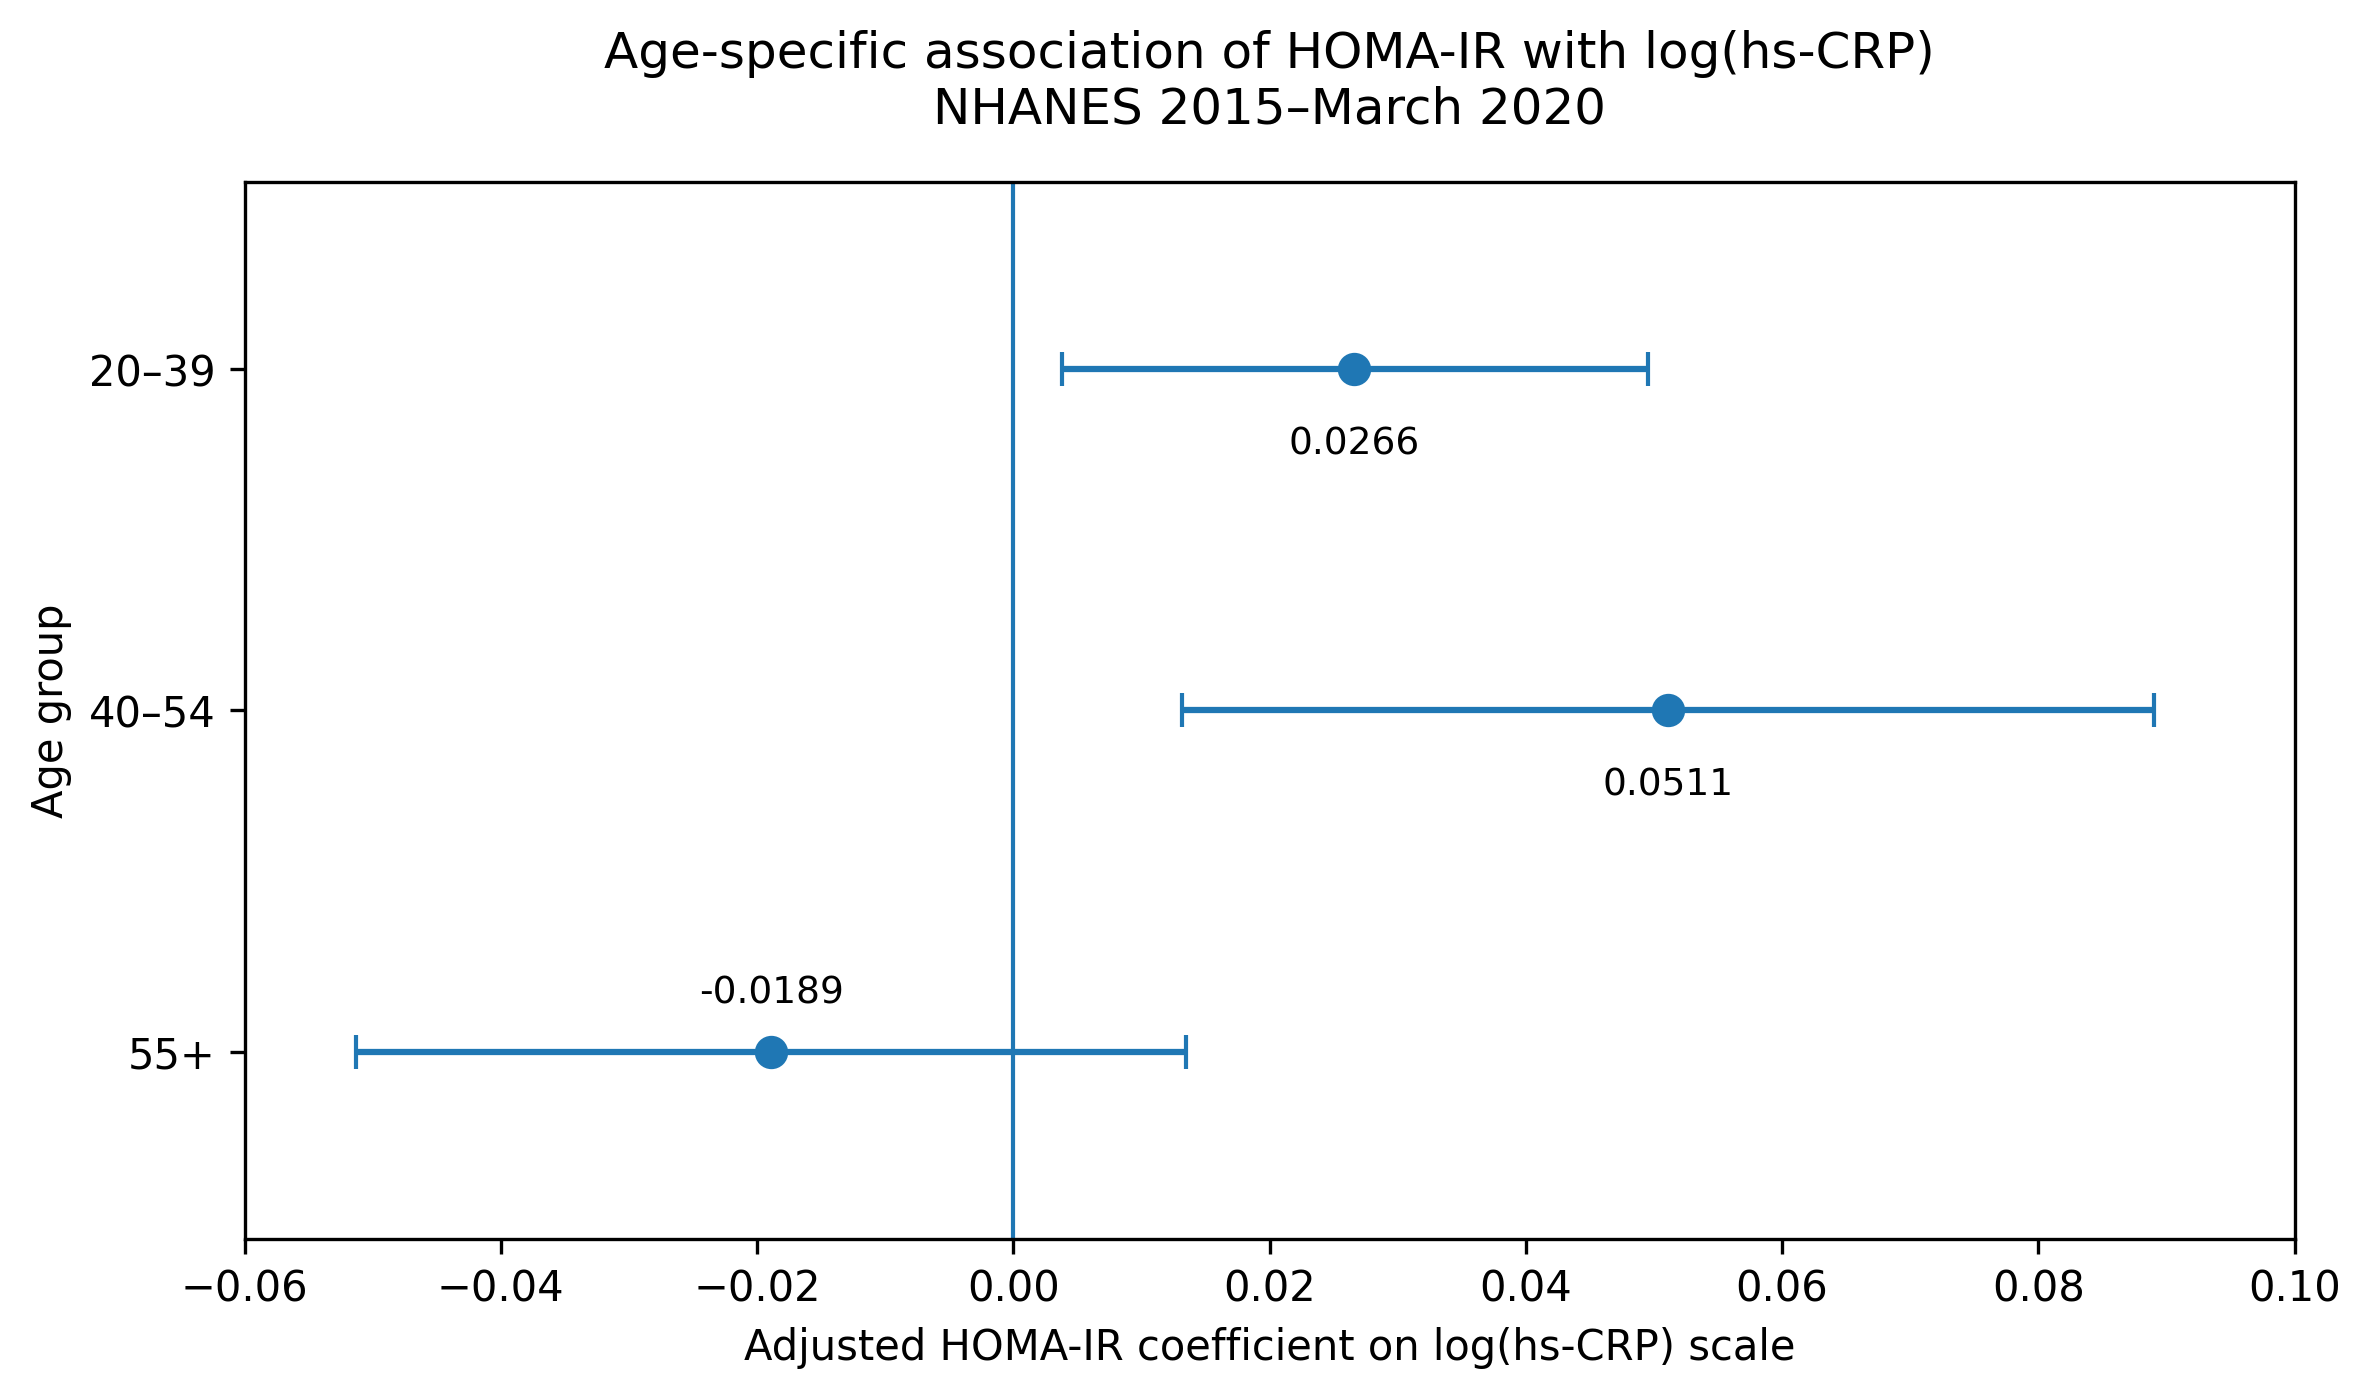
\includegraphics[width=0.78\textwidth]
    {age_group_HOMA_effect_forest_2015_2020.png}
    \caption{
    Adjusted age-specific associations between HOMA-IR and
    log-transformed hs-CRP in U.S. adults with HbA1c $<5.7\%$,
    NHANES 2015--March 2020. Points represent estimated HOMA-IR
    coefficients and horizontal bars represent 95\% confidence
    intervals. Estimates were obtained from the primary
    survey-adjusted interaction model controlling for HbA1c,
    waist circumference, continuous age, sex, and non-HDL
    cholesterol. The vertical reference line denotes a coefficient
    of zero.
    }
    \label{fig:agegroups}
\end{figure}


\subsection{Continuous-Age Analysis}

Continuous-age analyses were performed to determine whether the
observed effect modification depended on the prespecified age-group
boundaries. A model imposing a linear HOMA-IR-by-age interaction
provided borderline evidence of age modification,

\[
F(1,40)=3.93,
\qquad
p=0.054.
\]

Allowing the relationship to vary quadratically strengthened the
evidence for age modification,

\[
F(2,40)=3.43,
\qquad
p=0.042,
\]

although the additional quadratic interaction component considered
separately did not provide strong evidence for a specifically
quadratic functional form ($p=0.086$).

A four-degree-of-freedom natural cubic spline model also supported
age-dependent variation in the HOMA-IR association,

\[
F(4,40)=3.09,
\qquad
p=0.026.
\]

As shown in Figure~\ref{fig:spline}, the estimated HOMA-IR coefficient
remained positive through early and middle adulthood and subsequently
attenuated with increasing age. The spline was used to characterize
the continuous shape of the interaction rather than to identify a
specific age threshold.

\begin{figure}[htbp]
    \centering
    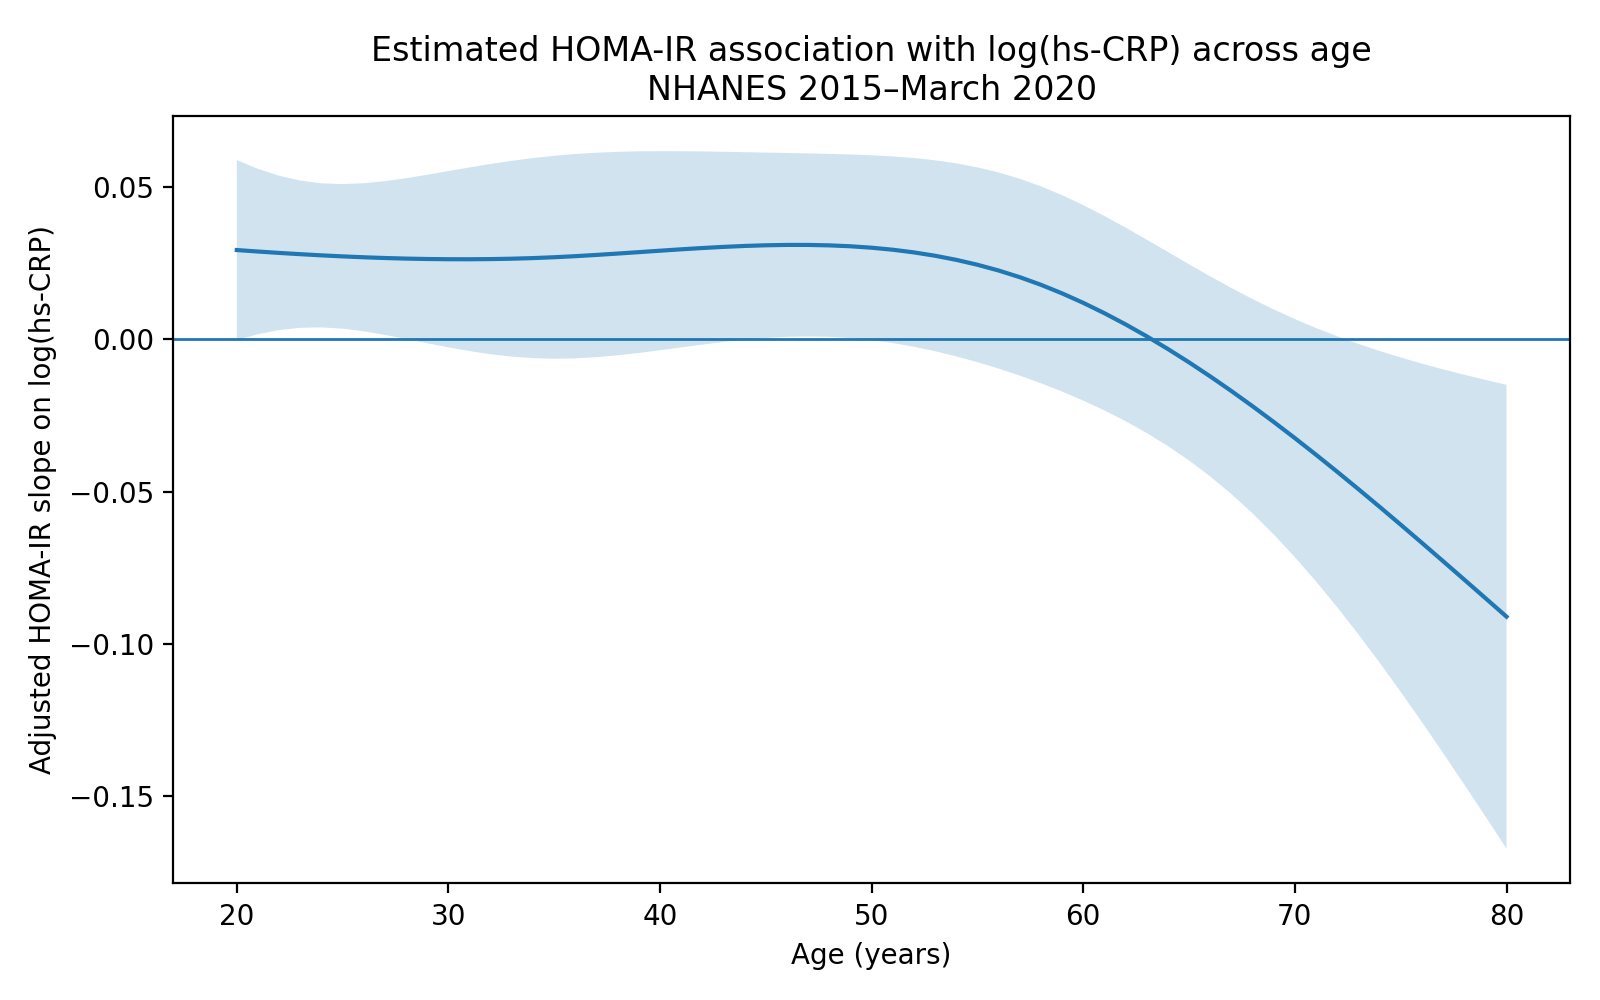
\includegraphics[width=0.82\textwidth]
    {continuous_age_spline_HOMA_effect_2015_2020.png}
    \caption{
    Estimated age-varying association between HOMA-IR and
    log-transformed hs-CRP in U.S. adults with HbA1c $<5.7\%$,
    NHANES 2015--March 2020. The solid curve represents the
    estimated adjusted HOMA-IR coefficient as a continuous function
    of age, and the shaded region represents the 95\% confidence
    interval. The horizontal reference line denotes no association.
    The curve represents variation in the HOMA-IR--hs-CRP
    association with age and does not represent the age trajectory
    of hs-CRP itself.
    }
    \label{fig:spline}
\end{figure}


\subsection{Independent-Cycle Replication}

The age-dependent association was additionally evaluated in the
independent 2015--2016 and 2017--2018 NHANES cycles using harmonized
waist-adjusted models. On the raw hs-CRP scale, the formal
HOMA-IR-by-age interaction was significant in both 2015--2016,

\[
F(2,15)=4.48,
\qquad
p=0.0298,
\]

and 2017--2018,

\[
F(2,15)=7.26,
\qquad
p=0.00625.
\]

The raw-scale HOMA-IR coefficients for the 20--39, 40--54, and
55+ year age groups were, respectively, 0.114, 0.329, and $-0.028$
in 2015--2016 and 0.298, 0.229, and $-0.341$ in 2017--2018.

A formal HOMA-IR-by-age-group-by-cycle interaction did not provide
strong evidence that the age-dependent pattern differed between the
two cycles,

\[
F(2,30)=2.22,
\qquad
p=0.126.
\]

The replication analysis was also repeated using log-transformed
hs-CRP. The age-specific log-scale HOMA-IR coefficients for
2015--2016 and 2017--2018, respectively, were 0.025 and 0.036 among
adults aged 20--39 years, 0.074 and 0.057 among adults aged
40--54 years, and $-0.030$ and $-0.063$ among adults aged 55 years
or older.

On the log scale, the formal cross-cycle heterogeneity test yielded

\[
F(2,30)=0.586,
\qquad
p=0.563.
\]

The corresponding direct cross-cycle comparisons gave $p=0.741$,
$p=0.659$, and $p=0.373$ for the young, midlife, and older age
groups, respectively. Thus, the data did not provide evidence that
the age-specific HOMA-IR associations differed between the two
independent survey cycles.

\subsection{Sensitivity and Robustness Analyses}

The primary finding was evaluated across alternative outcome and exposure
scales, restrictions on inflammatory extremes, alternative adiposity
adjustment, alternative HbA1c eligibility criteria, continuous-age
specifications, and survey-cluster influence. Detailed results are
presented in Supplementary Table~S1.

When hs-CRP was analyzed on its original scale in the combined
2015--March 2020 population, evidence of age modification remained,

\[
F(2,40)=3.96,
\qquad
p=0.0269.
\]

The corresponding raw-scale HOMA-IR coefficients were 0.127
(95\% CI, 0.018 to 0.235) among adults aged 20--39 years,
0.160 (95\% CI, $-0.056$ to 0.377) among adults aged
40--54 years, and $-0.109$ (95\% CI, $-0.282$ to 0.064)
among adults aged 55 years or older.

Evidence for interaction was less pronounced when HOMA-IR was
log-transformed. With log-transformed hs-CRP as the outcome, the
HOMA-IR-by-age interaction yielded

\[
F(2,40)=1.86,
\qquad
p=0.169,
\]

and when log-transformed HOMA-IR was combined with untransformed
hs-CRP, the interaction yielded

\[
F(2,40)=1.43,
\qquad
p=0.251.
\]

Thus, the qualitative age-specific pattern remained recognizable
across exposure and outcome transformations, but the strength of
formal interaction evidence varied across scale specifications.

Restriction of hs-CRP to values $\leq10$ mg/L produced a similar
distinction between outcome scales. With untransformed hs-CRP,
evidence of age modification remained,

\[
F(2,40)=4.03,
\qquad
p=0.0255,
\]

with age-specific HOMA-IR coefficients of 0.0824, 0.0905, and
$-0.0304$ among adults aged 20--39, 40--54, and 55 years or older,
respectively. With log-transformed hs-CRP under the same restriction,
the corresponding interaction was attenuated,

\[
F(2,40)=2.58,
\qquad
p=0.0883.
\]

\paragraph{Alternative adiposity specifications.}
The age-dependent HOMA-IR--hs-CRP association was not specific to the use
of waist circumference as the primary adiposity covariate. In a common
analytic sample with complete waist circumference, BMI, and
waist-to-height ratio data ($n=3{,}072$), the HOMA-IR-by-age interaction
remained significant when the primary model was adjusted for waist
circumference ($p=0.0066$), BMI ($p=0.0124$), or waist-to-height ratio
($p=0.0023$). Across all three specifications, the adjusted HOMA-IR
association remained positive among adults aged 20--39 and 40--54 years
and was substantially attenuated among adults aged $\geq55$ years.

Waist-to-hip ratio could be evaluated only during the survey period in
which hip circumference was available. Within a common sample from that
period ($n=1{,}899$), formal evidence for age modification was weaker
across adiposity specifications, including waist circumference.
Adjustment for waist-to-hip ratio produced less attenuation of the
HOMA-IR association among adults aged $\geq55$ years than did adjustment
for waist circumference, BMI, or waist-to-height ratio
(Supplementary Table~S2).

The findings were insensitive to the dual use of HbA1c as an
eligibility criterion and an adjustment covariate. When continuous
HbA1c was removed from the model while retaining the HbA1c $<5.7\%$
eligibility criterion, the HOMA-IR-by-age interaction was essentially
unchanged,

\[
F(2,40)=5.57,
\qquad
p=0.00732.
\]

The corresponding HOMA-IR coefficients were 0.0284, 0.0521, and
$-0.0171$ among adults aged 20--39, 40--54, and 55 years or older,
respectively, compared with 0.0266, 0.0511, and $-0.0189$ in the
primary model.

The age interaction also persisted when the HbA1c eligibility
criterion was progressively relaxed. The interaction yielded

\[
F(2,40)=5.74,\qquad p=0.00644
\]

for HbA1c $<6.0\%$;

\[
F(2,40)=5.58,\qquad p=0.00731
\]

for HbA1c $<6.5\%$; and

\[
F(2,40)=5.74,\qquad p=0.00643
\]

when the HbA1c eligibility threshold was removed while participants
with diagnosed diabetes remained excluded. These analyses indicate
that the observed age modification was not explained solely by
selection at the 5.7\% HbA1c threshold.

Alternative continuous-age specifications provided complementary
evidence. As reported above, the linear interaction yielded
$p=0.0544$, the joint quadratic interaction yielded $p=0.0421$,
and the four-degree-of-freedom natural cubic spline interaction
yielded $p=0.0262$, indicating that evidence for age modification
was stronger when nonlinear variation across adulthood was permitted.

The expanded combined-period analysis additionally tested whether
the age-dependent HOMA-IR association differed between the
2015--2016 and 2017--March 2020 components. For the primary
log-hs-CRP specification, the period heterogeneity test yielded

\[
F(2,40)=0.728,
\qquad
p=0.489,
\]

providing no strong evidence of between-period heterogeneity in the
age-dependent association.

Finally, leave-one-survey-cluster-out analysis generated 79 refitted
models after sequential removal of each unique masked
stratum--PSU combination. Across these refits, the HOMA-IR-by-age
interaction $F$ statistic ranged from 3.59 to 7.66, with corresponding
$p$-values ranging from 0.00157 to 0.0369. No single masked
stratum--PSU cluster eliminated evidence of the interaction.

Additional supportive analyses conducted during the methodological
audit evaluated influential observations, smoking, medication burden,
statin use, renal and liver/metabolic biochemical variables, expanded
covariate sets, and sex heterogeneity. These exploratory analyses did
not identify an obvious single factor accounting for the overall
age-dependent pattern and were not treated as additional primary
hypothesis tests.

\subsection{Use of Generative Artificial Intelligence}

Generative artificial intelligence (ChatGPT, OpenAI) was used extensively
as a research-support tool during this project, including assistance with
drafting and revising portions of the manuscript and with writing,
optimizing, and debugging portions of the reproducible Python analysis
pipeline. The authors determined the research questions, analytic strategy,
statistical methods, interpretation of results, and conclusions. AI-assisted
analytical code and outputs were subject to human review and validation
against the prespecified analytic framework, mathematical expectations,
and NHANES survey-design constraints. The primary analysis was additionally
reproduced independently in R as a cross-software validation. All manuscript
content was critically reviewed and approved by the authors, who take full
responsibility for the accuracy, integrity, interpretation, and conclusions
of the work.

% ============================================================

\section{Discussion}

\subsection{Principal Findings}

In this nationally representative analysis of U.S. adults without
diagnosed diabetes and with HbA1c below 5.7\%, HOMA-IR was associated
with systemic inflammatory status in an age-dependent manner. In the
primary 2015--March 2020 analysis, the adjusted association between
HOMA-IR and log-transformed hs-CRP differed across age groups. Higher
HOMA-IR was associated with higher hs-CRP among adults aged 20--39 years
and more strongly among those aged 40--54 years, whereas the corresponding
association among adults aged 55 years or older was attenuated and
statistically indistinguishable from zero.

Importantly, the evidence for age modification arose from a formal
interaction test rather than from comparison of statistical significance
across separately fitted age-stratified models. The age-dependent pattern
was statistically compatible across the independent 2015--2016 and
2017--2018 NHANES cycles, and continuous-age modeling produced a broadly
consistent pattern in which the estimated HOMA-IR association remained
positive through early and middle adulthood and weakened later in
adulthood.

The qualitative age-dependent pattern was generally recognizable across
multiple sensitivity analyses addressing outcome transformation,
inflammatory extremes, exposure scale, adiposity specification, HbA1c
eligibility, additional covariates, and influential survey clusters.
However, the strength of formal interaction evidence varied across
specifications, particularly when HOMA-IR was log-transformed or when
log-transformed hs-CRP was analyzed after restriction to hs-CRP
$\leq10$ mg/L. The overall evidence therefore supports age-dependent
heterogeneity in the HOMA-IR--hs-CRP association while also indicating
that the estimated strength of effect modification is sensitive to
modeling scale.


\subsection{Insulin Resistance and Inflammation Below Conventional
Glycemic Thresholds}

The association between insulin resistance and systemic inflammation is
not itself a novel observation. Previous population-based studies,
including analyses of U.S. NHANES data and other national and longitudinal
cohorts, have reported associations between HOMA-IR or fasting insulin and
C-reactive protein in adults without diabetes
\citep{Chen2004,Meng2007,Park2009,Missel2021}. Related studies have also
demonstrated substantial metabolic heterogeneity among individuals without
overt dysglycemia \citep{Caporaso2020}.

The present study addresses a narrower question. Rather than asking simply
whether insulin resistance is associated with inflammation, we restricted
the primary population to adults remaining below the conventional HbA1c
prediabetes threshold of 5.7\% \citep{ADA2026Diagnosis} and examined whether
the strength of the HOMA-IR--hs-CRP association itself varied across
adulthood. Prior work has examined demographic heterogeneity in
insulin resistance--inflammation associations, including nationally
representative studies evaluating sex and age
\citep{Caporaso2020,Shahid2023}. Comparatively less evidence, however, has
focused specifically on formal age modification of this relationship within
a population remaining below the conventional HbA1c prediabetes threshold.

This distinction matters because HbA1c and HOMA-IR characterize different
aspects of metabolic physiology. HbA1c summarizes glycemic exposure
\citep{Nathan2007,ADA2026Diagnosis}, whereas HOMA-IR estimates insulin
resistance from the fasting glucose--insulin relationship
\citep{Matthews1985,Wallace2004}. During compensatory stages of insulin
resistance, increased insulin secretion may contribute to maintenance of
glucose concentrations despite diminished insulin sensitivity
\citep{Rodzen2026}. Consequently, similar HbA1c values need not imply
similar insulin dynamics.

Consistent with this distinction, HOMA-IR values in the present analytic
population were not concentrated at a single level despite restriction to
HbA1c below 5.7\%. Moreover, survey-weighted median HOMA-IR was relatively
similar across the three age groups, even though the estimated relationship
between HOMA-IR and hs-CRP differed substantially by age. The age-dependent
association therefore should not be interpreted simply as a consequence of
middle-aged adults having higher average HOMA-IR than the other age groups.

The present findings are thus consistent with meaningful metabolic
heterogeneity within an HbA1c-defined population that remains below the
prediabetes threshold. They do not establish that such heterogeneity is
pathological in every individual, but they indicate that glycemic
classification alone does not fully characterize variation in insulin
resistance or its relationship with systemic inflammatory status.

\subsection{Age Modification}

Age modification was not the original hypothesis motivating this study.
The initial scientific question concerned whether HOMA-IR identified
inflammatory heterogeneity among adults remaining below the conventional
HbA1c prediabetes threshold. The age-dependent pattern emerged during
evaluation of the initial stratified analyses and was subsequently subjected
to formal interaction testing, independent-cycle replication,
continuous-age modeling, and sensitivity analyses. Accordingly, the
specific shape of the age-dependent association should be interpreted as
an empirically identified and subsequently robustness-tested finding rather
than as a prospectively specified biological prediction.

Age modification is a central finding of the present analysis. In the
primary model, the HOMA-IR--hs-CRP association was positive in younger
adults, strongest in the 40--54-year group, and attenuated among adults
aged 55 years or older. Continuous-age modeling provided additional evidence
that the phenomenon is not well described by a constant HOMA-IR effect
across the adult lifespan.

This pattern should not be interpreted as evidence that hs-CRP declines
with age. The interaction describes how the adjusted association between
HOMA-IR and hs-CRP changes with age, not how hs-CRP itself changes with
age. Indeed, median hs-CRP was modestly higher in the oldest age group.
Nor should the spline be interpreted as identifying a discrete biological
age at which the association disappears. The continuous-age results are
more consistent with gradual variation in the strength of the association
across adulthood.

The mechanism underlying the older-age attenuation cannot be determined
from the present study. One possibility is that the relative contribution
of insulin resistance to systemic inflammatory variation changes as
inflammatory, adipose, metabolic, and cellular processes evolve with age
\citep{Park2014AgingIR}. Medication exposure, comorbidity burden, lifestyle
changes, and other determinants of inflammatory status may add further
heterogeneity later in life, although the present study cannot determine
the contribution of these factors. Such processes could reduce the extent
to which variation in HOMA-IR tracks variation in hs-CRP even if overall
inflammatory burden remains elevated.

Selection may also contribute. Because the present analysis intentionally
excludes individuals with diagnosed diabetes and those with HbA1c at or
above 5.7\%, the meaning of remaining in the analytic population changes
with age. An older participant who continues to satisfy these criteria may
differ systematically from a peer who previously crossed a glycemic
threshold or developed diagnosed diabetes and was therefore excluded.

However, sensitivity analyses progressively relaxing the HbA1c eligibility
criterion to $<6.0\%$, $<6.5\%$, and ultimately no HbA1c cutoff did not
restore a positive older-adult HOMA-IR--hs-CRP association. This finding
argues against a simple explanation in which the older-age attenuation is
produced solely by exclusion at the 5.7\% HbA1c threshold. It does not,
however, eliminate broader selection effects or distinguish them from
biological effect modification, treatment effects, cohort differences,
behavioral adaptation, residual confounding, or combinations of these
processes.

The data therefore establish attenuation of an association; they do not
establish why that attenuation occurs. Similarly, the older-adult point
estimate should not be interpreted as evidence of a protective relationship
between insulin resistance and inflammation.

The role of adiposity warrants particular consideration. In unadjusted
analyses, HOMA-IR was positively associated with hs-CRP across all three
age groups, whereas adjustment for waist circumference accounted for most
of the transition to the age-dependent pattern observed in the primary
model. Importantly, however, this pattern was not specific to waist
circumference. In common-sample analyses spanning the full study period,
substitution of either BMI or waist-to-height ratio for waist circumference
produced the same qualitative pattern of positive associations in early
and middle adulthood and marked attenuation in older adults. Thus, the
observed age-dependent pattern appears to depend importantly on
accounting for adiposity, but not on a single full-period anthropometric
measure.

These findings should not be interpreted as showing that adiposity simply
confounds an otherwise causal association between insulin resistance and
inflammation. Central adiposity, insulin resistance, and inflammatory
signaling are biologically interrelated, and their temporal and causal
relationships cannot be resolved in cross-sectional data. Waist
circumference may therefore represent an upstream determinant, an
intermediate phenotype, a correlate of shared metabolic processes, or
some combination of these roles. The adjusted estimates are consequently
best interpreted as conditional associations describing variation in
inflammatory status associated with HOMA-IR among individuals with similar
measured adiposity and other model covariates.

In the restricted survey period in which waist-to-hip ratio was available,
the older-age association was less attenuated after adjustment for
waist-to-hip ratio than after adjustment for the other anthropometric
measures; however, evidence for age modification was generally weaker in
this restricted sample even when waist circumference was retained.

The observed age modification was also insensitive to whether continuous
HbA1c was retained as an adjustment covariate after restriction to
HbA1c $<5.7\%$. Removing continuous HbA1c produced age-specific coefficients
that were nearly identical to those in the primary model, indicating that
the principal finding was not driven by the dual role of HbA1c in population
definition and covariate adjustment.

\subsection{Reconsidering the Metabolic ``Blind Spot''}

The results permit a more precise formulation of the metabolic ``blind
spot'' that motivated this study. We do not use the term to suggest that
HbA1c is an inadequate measure of glycemia, nor do the findings imply that
individuals with HbA1c below 5.7\% should be considered metabolically
abnormal solely because they have a higher HOMA-IR.

Rather, the blind spot is one of \emph{measurement domain}. HbA1c answers
a question about glycemic exposure \citep{Nathan2007,ADA2026Diagnosis}. It does not directly measure the amount
of insulin required to maintain that glycemic state or the degree of tissue
insulin sensitivity \citep{Matthews1985,Wallace2004}. Two individuals can therefore occupy the same
HbA1c-defined category while differing substantially in fasting insulin
and HOMA-IR.

The original hypothesis of the study was therefore supported in a qualified
rather than universal sense. Among adults remaining below the conventional
HbA1c prediabetes threshold, variation in HOMA-IR was associated with
variation in systemic inflammatory status. However, this relationship was
not uniform across adulthood. The evidence was strongest in early and
middle adulthood and attenuated in the older group.

This refinement is important. The relevant inference is not that HbA1c
``misses disease,'' but that an HbA1c value below 5.7\% does not define a
metabolically homogeneous population. HOMA-IR captures variation in insulin
dynamics that is not represented directly by HbA1c, and at least some of
that variation is associated with systemic inflammatory status.

The distinction may be more useful than framing HOMA-IR and HbA1c as
competing biomarkers. They measure different features of metabolic
regulation. The clinically relevant question is therefore not whether
HOMA-IR should replace HbA1c, but whether direct information about insulin
resistance adds useful predictive or decision-relevant information to
conventional glycemic assessment in selected populations.


\subsection{Clinical and Public-Health Implications}

Recent reviews have called for improved recognition and characterization
of insulin resistance before the development of overt metabolic disease
and have emphasized the absence of standardized criteria for its routine
clinical identification \citep{Rodzen2026}. The present findings are relevant to that broader
discussion because they demonstrate measurable heterogeneity in insulin
resistance and its inflammatory correlates among adults who remain below
the conventional HbA1c prediabetes threshold.

The present study does not, however, establish the clinical utility of
routine fasting insulin measurement, and our findings alone do not justify
changing screening recommendations. A cross-sectional association with
hs-CRP is insufficient to demonstrate that measuring HOMA-IR improves
prediction, alters clinical decision-making, or ultimately improves patient
outcomes.

The findings instead provide a rationale for prospective evaluation of
those questions. Future studies could test whether incorporating fasting
insulin or validated measures of insulin resistance into risk assessment
improves prediction beyond HbA1c, fasting glucose, anthropometry, lipids,
and established clinical risk factors. Longitudinal studies would be
particularly valuable for clarifying temporal relationships between insulin
resistance, inflammation, and subsequent metabolic risk
\citep{Park2009,Yan2019}, including whether individuals with higher HOMA-IR
but HbA1c below 5.7\% are at increased risk of subsequent dysglycemia,
cardiovascular events, metabolic liver disease, or other clinically
relevant outcomes.

Such work should also evaluate whether predictive utility varies by age.
The present analysis suggests that the relationship between insulin
resistance and inflammatory status is not uniform across adulthood.
Accordingly, even if additional insulin-resistance measurement ultimately
proves clinically informative, there is no basis for assuming that the
same threshold, interpretation, or screening strategy would necessarily
perform equivalently across age groups.

This perspective is consistent with recent calls for improved diagnostic
frameworks for insulin resistance while also emphasizing the need for
empirical validation before policy or screening recommendations are
changed. The present study contributes population-level evidence relevant
to that discussion but does not resolve the clinical-policy question.


\subsection{Strengths and Limitations}

This study has several strengths. The primary analysis uses a large,
nationally representative pre-pandemic NHANES population and incorporates
the fasting-subsample weights, stratification, and clustering required for
design-based inference. The age-dependent pattern identified during
methodological evaluation was subsequently tested using a formal
HOMA-IR-by-age interaction rather than by comparing subgroup $p$-values.

The analysis also provides several complementary assessments of
reproducibility and robustness. The age-dependent pattern was evaluated
across independent conventional NHANES cycles, examined continuously using
linear, quadratic, and spline-based age specifications, and subjected to
sensitivity analyses addressing outcome and exposure scale, inflammatory
extremes, adiposity adjustment, HbA1c eligibility, and survey-cluster
influence. No single masked stratum--PSU cluster eliminated evidence of the
primary interaction. Importantly, not every alternative specification
produced equally strong formal interaction evidence, and these results are
reported rather than excluded from consideration.

Several limitations are equally important. First, NHANES is cross-sectional;
temporal ordering between insulin resistance and inflammation cannot be
established. The observed association therefore cannot determine whether
insulin resistance contributes to inflammation, inflammation contributes
to insulin resistance, both arise from shared upstream processes, or some
combination of these mechanisms operates.

Second, HOMA-IR is a surrogate measure derived from fasting glucose and
insulin rather than a direct measurement of insulin sensitivity such as the
hyperinsulinemic-euglycemic clamp \citep{DeFronzo1979,Wallace2004}. Although
it is widely used in population research and correlates with more intensive
physiological measures, measurement error and biological variability
remain.

Third, hs-CRP is a nonspecific marker of systemic inflammation and can be
influenced by infection, chronic inflammatory conditions, adiposity,
medication use, and other factors unrelated to insulin resistance \citep{Pepys2003}.
Sensitivity analyses limiting extreme hs-CRP values and adjusting for
additional available covariates reduce but cannot eliminate this concern.

Fourth, formal evidence for effect modification varied across model
specifications. Although the qualitative pattern of positive associations
earlier in adulthood and attenuation later in adulthood was generally
recognizable, interaction tests were weaker under some exposure and outcome
transformations. The magnitude and statistical strength of age modification
should therefore not be regarded as invariant to modeling scale.

Fifth, residual and unmeasured confounding remain possible despite
adjustment for HbA1c, adiposity, sex, age, and non-HDL cholesterol and
the additional sensitivity analyses. Although the age-dependent pattern
was reproduced using multiple anthropometric specifications, these
measures are imperfect proxies for body composition and fat distribution
and cannot fully account for the complex relationship between adiposity,
insulin resistance, and inflammation.

Sixth, the primary analysis used complete cases, creating the possibility
of selection bias if missingness was related to the exposure, outcome, or
covariates under study. However, only 103 of 3,182 participants (3.2\%)
who otherwise met the eligibility and measurement requirements were
excluded because of incomplete primary-model covariate data. The small
proportion of exclusions limits, but does not eliminate, this concern.

Seventh, restricting the primary study population to participants without
diagnosed diabetes and with HbA1c below 5.7\% creates a deliberately
selected analytic population. This restriction is essential to the
scientific question but complicates interpretation of age differences
because older adults remaining below the threshold may not be directly
comparable, in a life-course sense, with younger adults meeting the same
criteria.

The use of NHANES probability sampling and appropriate fasting-subsample
weights supports population-level inference to the noninstitutionalized
U.S. adult population meeting the study eligibility criteria. The findings
should not, however, be assumed to generalize to institutionalized
populations, populations outside the United States, individuals with
diagnosed diabetes or HbA1c $\geq5.7\%$, or populations whose metabolic
and inflammatory characteristics differ substantially from those
represented in NHANES.

Finally, age modification was identified during methodological evaluation
rather than prospectively specified as the original study hypothesis.
Although the resulting pattern was subsequently subjected to formal
interaction testing, independent-cycle replication, continuous-age
modeling, and extensive sensitivity analysis, the precise age-dependent
shape should be regarded as a subsequently validated empirical observation
rather than a prospectively predicted biological pattern. The categorical
results likewise should not be interpreted as establishing a biological
threshold at age 55.

\subsection{Conclusion}

Among U.S. adults without diagnosed diabetes and with HbA1c below 5.7\%,
the adjusted association between HOMA-IR and systemic inflammatory status
varied across age. Higher HOMA-IR was associated with higher hs-CRP in
young and middle-aged adults, whereas the corresponding association was
attenuated among older adults. The age-dependent pattern was supported by
formal interaction testing, independent-cycle analyses, continuous-age
modeling, and multiple robustness analyses, although the strength of formal
interaction evidence varied across model specifications.

These findings support a qualified version of the original metabolic
``blind spot'' hypothesis: adults remaining below the conventional HbA1c
prediabetes threshold are not metabolically homogeneous, and variation in
insulin resistance can be associated with inflammatory physiology not fully
characterized by glycemic classification alone. The present data do not
establish whether this additional information improves prospective risk
prediction or clinical outcomes. Determining whether direct measurement of
insulin resistance adds clinically useful information to conventional
glycemic assessment, and whether that utility itself varies with age,
requires prospective investigation.

% ============================================================

\section*{Author Contributions}

S.M. conceived the study, developed the analytic framework, conducted
the statistical analyses, interpreted the results, and drafted the
manuscript. J.B. contributed to study development, interpretation of
the findings, and critical revision of the manuscript. Both authors
reviewed and approved the final manuscript.

\section*{Funding}

This research received no external funding.

\section*{Conflicts of Interest}

The authors declare no conflicts of interest.

\section*{Ethics Statement}

This study used publicly available, de-identified data from the National
Health and Nutrition Examination Survey (NHANES). NHANES protocols were
approved by the National Center for Health Statistics Research Ethics
Review Board, and written informed consent was obtained from participants
in accordance with NHANES procedures. Because the present study involved
secondary analysis of publicly available, de-identified data, no
additional institutional review board approval or informed consent was
required.

\section*{Data Availability}

The NHANES data used in this study are publicly available from the
National Center for Health Statistics.

% ============================================================
% References
% ============================================================

\bibliographystyle{plainnat}
\bibliography{manuscript_references}

\end{document}
